\subsubsection{22.11.14 (Competition)}
\begin{center}
	2-nd day of the competition "Robofest-South".
\end{center}
Today there were qualifying matches and protection of engineering books.
\newline 
Results of matches: 2 wins from 4. 
\newline
Results of protection of engineering books still unknown.
\newline
Main problems identified during matches:
\begin{enumerate}
	\item Low accuracy during throwing balls to the rolling goal. This was due to we didn't give enough time  to trainings.
	
	\item Because the wire of STB was fixed on the lift badly, it often hooked to slats and torned. Due to this it was impossible throw balls to baskets.
	
\end{enumerate} 
Improvisierents that were done:
\begin{enumerate}
	\item It was wrote programme of autonomous period, that includes exit from the ramp and throwing of autonomous balls to rolling goal 60cm.
	
	\item Because often there was the problem that after ending of programme the lift remains partially extend and we need to lower to it, there was wrote the programme that allows to control the lift by buttons of NXT. In addition this programme convenient if we need to extract the lift for working on the construction of robot.
	
	\item Also it was wrote the programme of autonomous period from the parking zone. It allows to knock down the fence if it is in the one position from three.
	
	\item Due to the high loads that that have experienced the crossbars, one from their bended so it was strengthened by the metallic tube from set Tetrix. It corrected this problem but it was decided to replace aluminium crossbars to steel when we'll return from the competition.
	
%	\begin{figure}[H]
%		\begin{minipage}[h]{0.2\linewidth}
%			\center  
%		\end{minipage}
%		\begin{minipage}[h]{0.6\linewidth}
%			\center{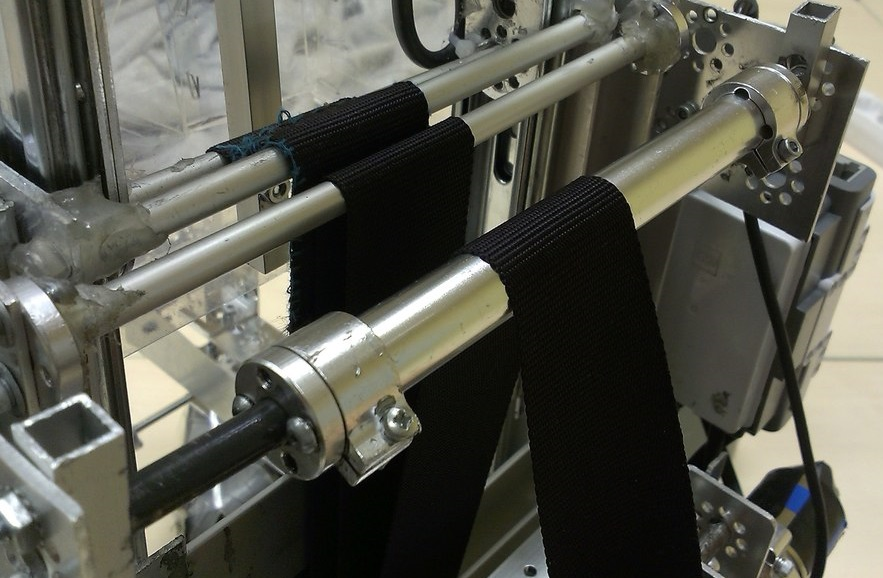
\includegraphics[scale=0.3]{days/22.11.14/images/01}}
%			\caption{Укрепление перекладины}
%		\end{minipage}
%	\end{figure}
	
	\item There was installed on MCB the slopes of the tie-rods for alignment of rolling goals. In the future we planned to replace the screeds  to plastic strips because they often broke.
	
	\begin{figure}[H]
		\begin{minipage}[h]{0.2\linewidth}
			\center  
		\end{minipage}
		\begin{minipage}[h]{0.6\linewidth}
			\center{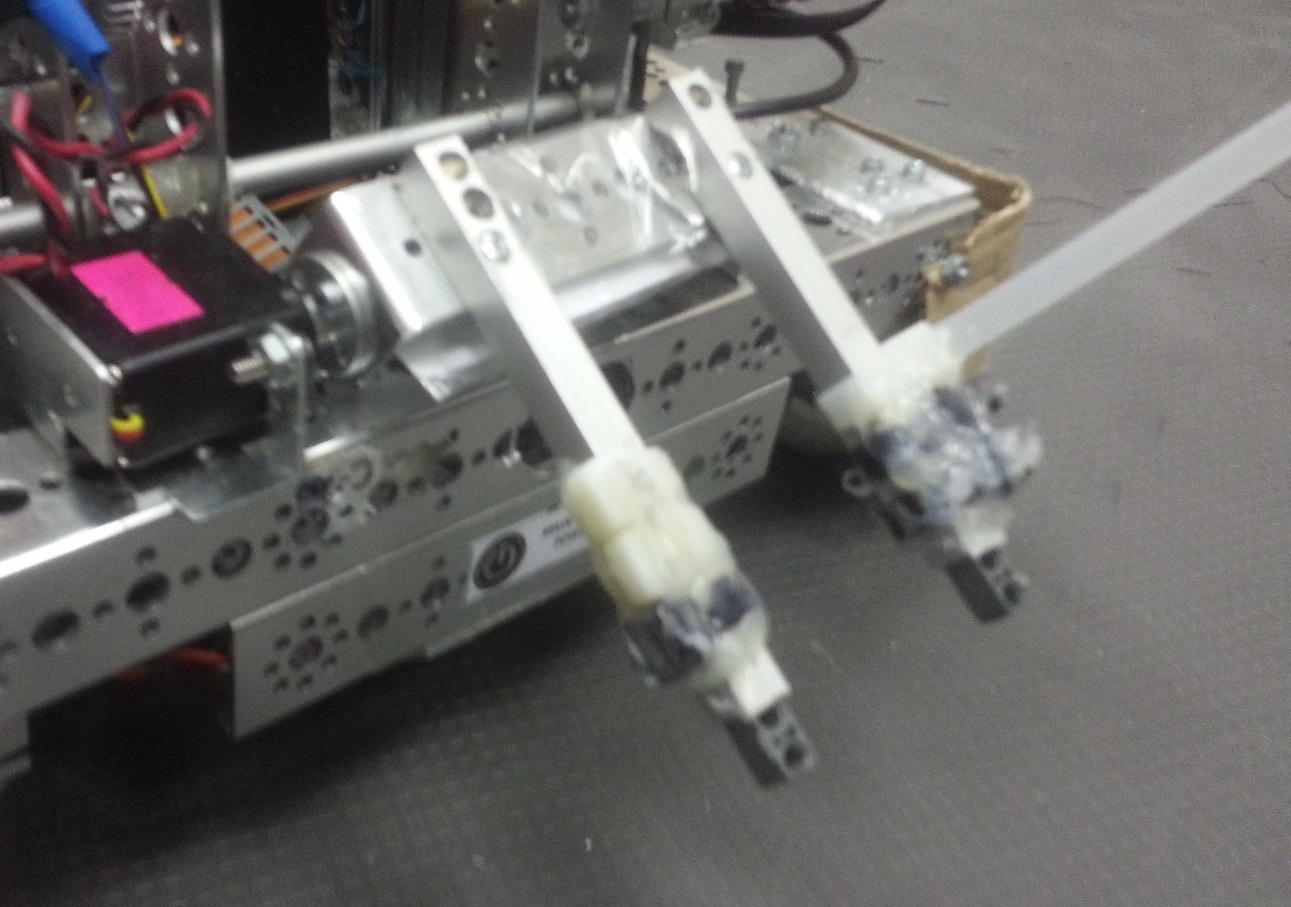
\includegraphics[scale=0.15]{days/22.11.14/images/02}}
			\caption {Slopes for alignment of rolling goals.}
		\end{minipage}
	\end{figure}
	
	\item Protection of wheels was improved . Now there is a cardboard protection but we planned make to it metallic.
	
	\begin{figure}[H]
		\begin{minipage}[h]{0.2\linewidth}
			\center  
		\end{minipage}
		\begin{minipage}[h]{0.6\linewidth}
			\center{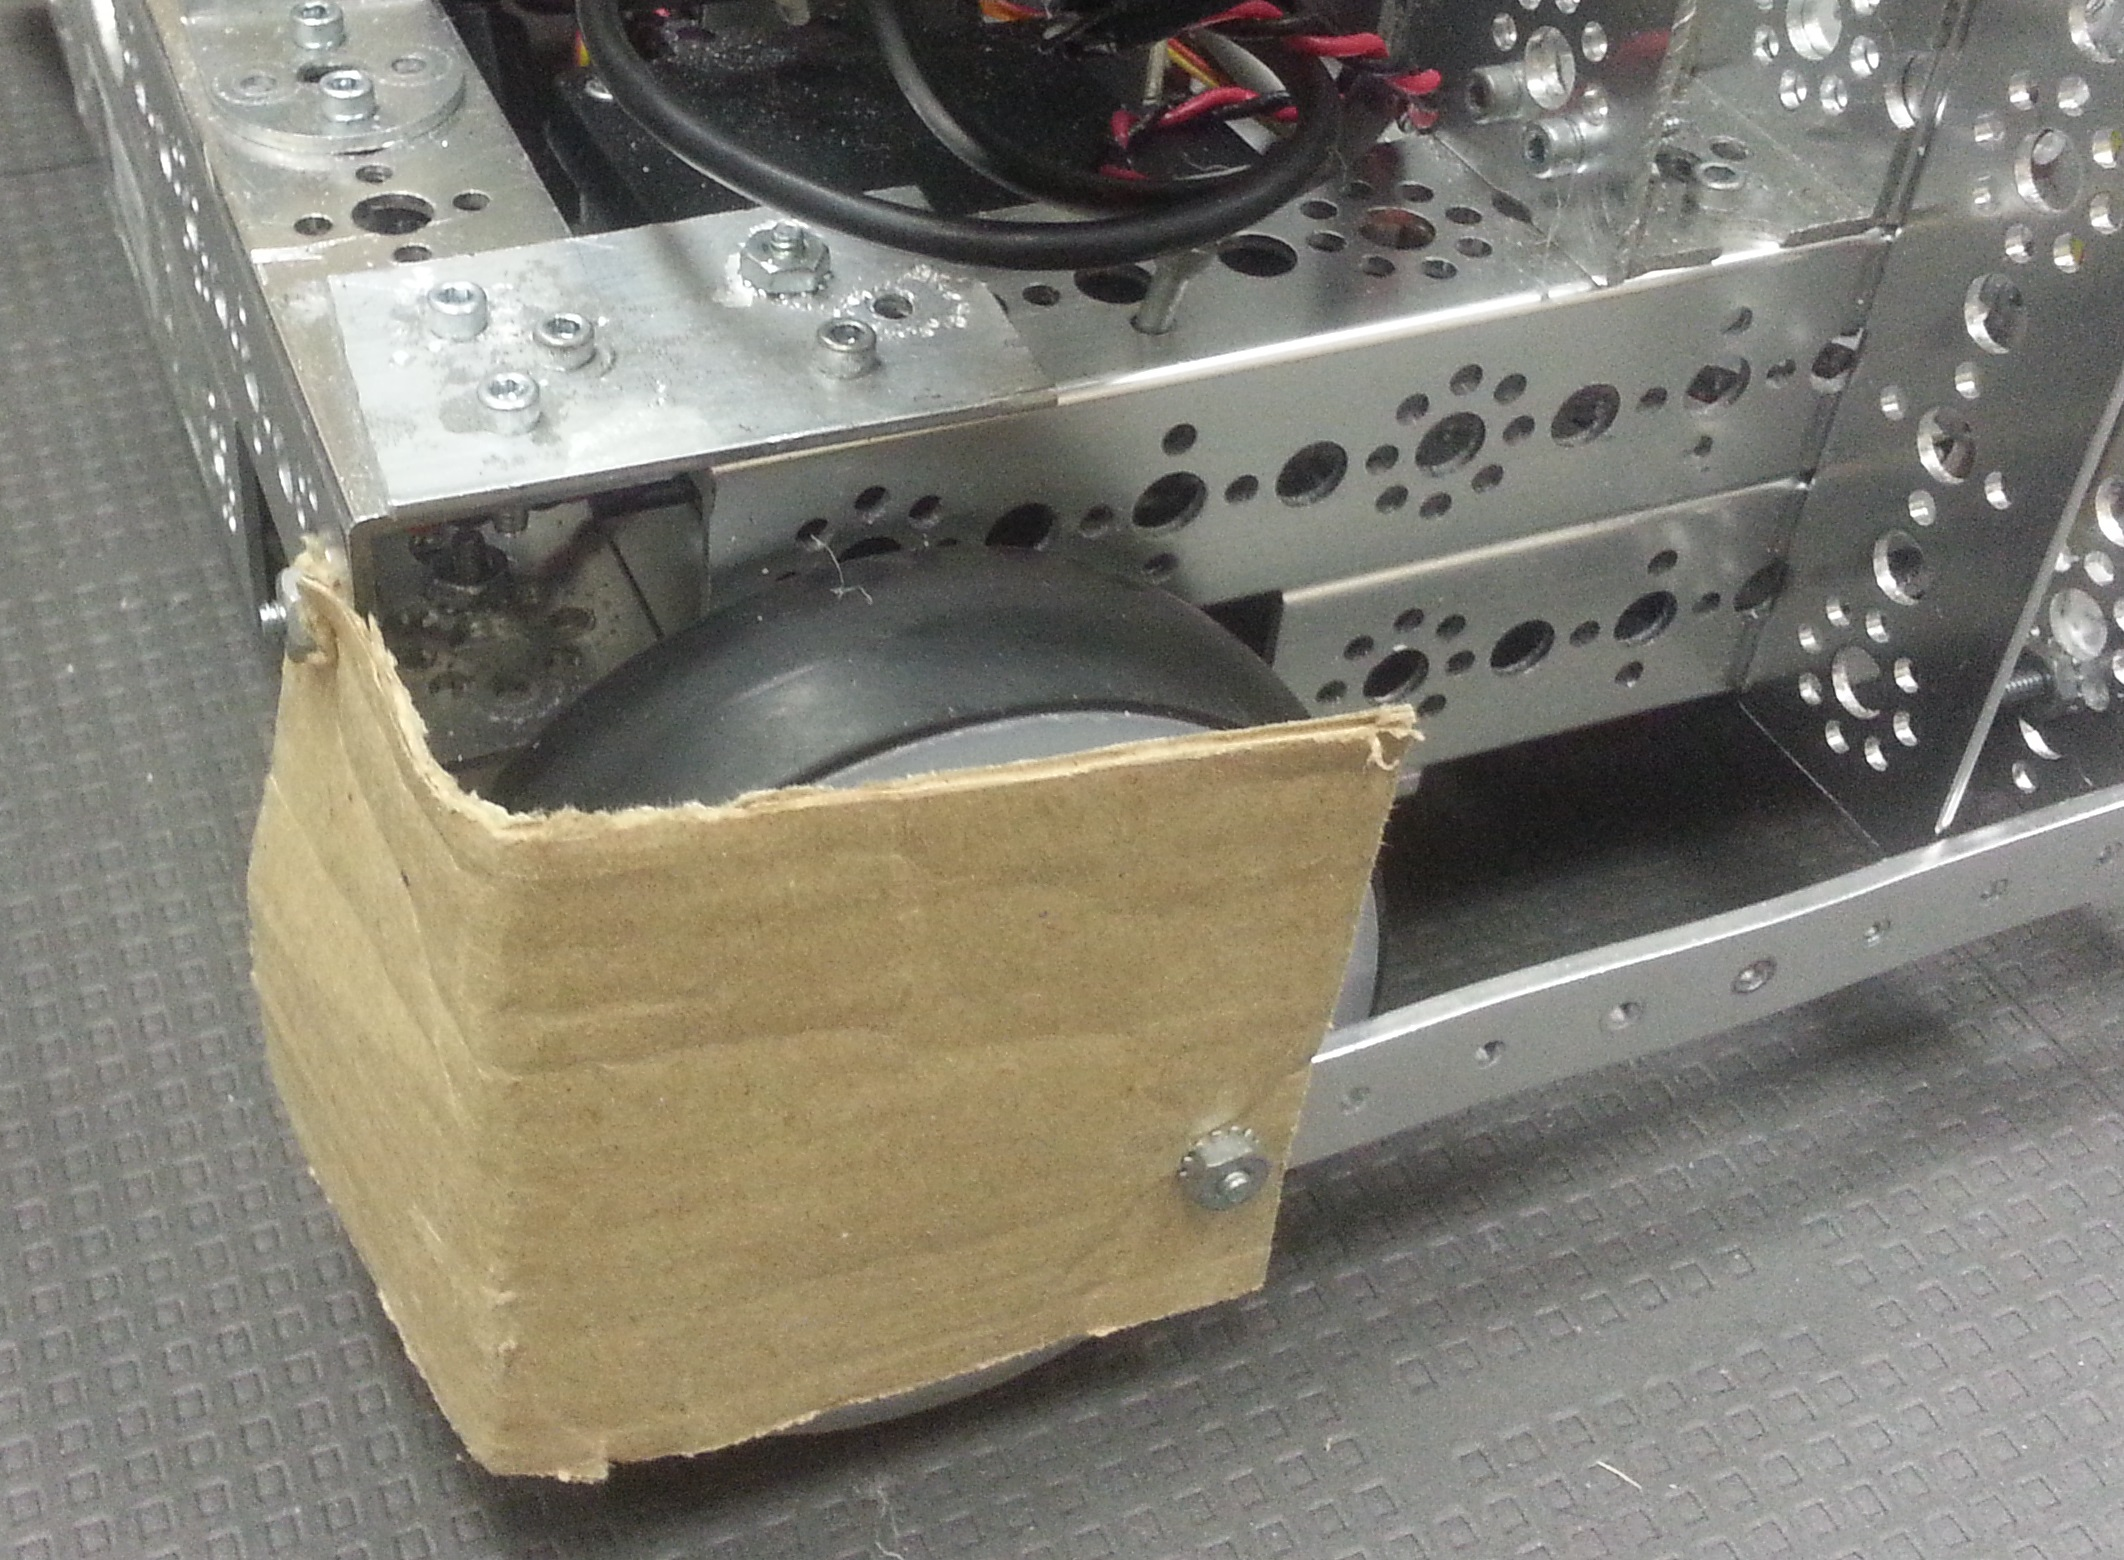
\includegraphics[scale=0.1]{days/22.11.14/images/03}}
			\caption{Protection of wheels}
		\end{minipage}
	\end{figure}
	
	\item Due to that during the one match NXT-brick fell off from the robot we fixed to it as effectively as possible.
	
	\begin{figure}[H]
		\begin{minipage}[h]{0.2\linewidth}
			\center  
		\end{minipage}
		\begin{minipage}[h]{0.6\linewidth}
			\center{
\includegraphics[scale=0.2]{days/22.11.14/images/04}}
			\caption{Improved fixing of NXT}
		\end{minipage}
	\end{figure}
	
	\item It was turned out that during extracting of the lift the top pair of slats rises the last. It doesn't allow to tilting the bucket up until the lift wasn't extracted fully. For throwing balls to any goal we must to extract the lift fully and then to lower this to needed heigh.Due to this problem we waste a lot of time so it was decided to correct this problems after returning from the competition.
	
\end{enumerate}
\fillpage